\documentclass{article}

% if you need to pass options to natbib, use, e.g.:
% \PassOptionsToPackage{numbers, compress}{natbib}
% before loading nips_2016
%
% to avoid loading the natbib package, add option nonatbib:
% \usepackage[nonatbib]{nips_2016}

% to compile a development version, don't pass any options.
% \usepackage{nips_2016}

% to compile a camera-ready version, add the [final] option, e.g.:
\usepackage[final]{nips_2016}

\usepackage[utf8]{inputenc} % allow utf-8 input
\usepackage[T1]{fontenc}    % use 8-bit T1 fonts
\usepackage{hyperref}       % hyperlinks
\usepackage{url}            % simple URL typesetting
\usepackage{booktabs}       % professional-quality tables
\usepackage{amsfonts}       % blackboard math symbols
\usepackage{nicefrac}       % compact symbols for 1/2, etc.
\usepackage{microtype}      % microtypography


\usepackage{color,graphicx}
\usepackage{lmodern}
\usepackage{hyperref}
\usepackage{amsmath}
\usepackage{amssymb}
\usepackage[T1]{fontenc}
\usepackage{fancyhdr}
\usepackage{color,graphicx}
\pagestyle{fancy}


\title{Assignment 4}

% The \author macro works with any number of authors. There are two
% commands used to separate the names and addresses of multiple
% authors: \And and \AND.
%
% Using \And between authors leaves it to LaTeX to determine where to
% break the lines. Using \AND forces a line break at that point. So,
% if LaTeX puts 3 of 4 authors names on the first line, and the last
% on the second line, try using \AND instead of \And before the third
% author name.

\author{
  Michele Cer\'u
  %\thanks{Use footnote for providing further
    %information about author (webpage, alternative
    %address)---\emph{not} for acknowledging funding agencies.} 
    \\
 % Department of Computer Science\\
  %Cranberry-Lemon University\\
  %Pittsburgh, PA 15213 \\
  \texttt{mc3784@nyu.edu} \\
}

\begin{document}
% \nipsfinalcopy is no longer used

\maketitle

%\begin{abstract}
 % The abstract paragraph should be indented \nicefrac{1}{2}~inch
  %(3~picas) on both the left- and right-hand margins. Use 10~point
  %type, with a vertical spacing (leading) of 11~points.  The word
  %\textbf{Abstract} must be centered, bold, and in point size 12. Two
  %line spaces precede the abstract. The abstract must be limited to
  %one paragraph.
%\end{abstract}

\section{nngraph}
\begin{enumerate}
\item the code for the first question (part a and b) is in \cite{wormup}.
%\begin{figure}[ht!]
  %\centering
  %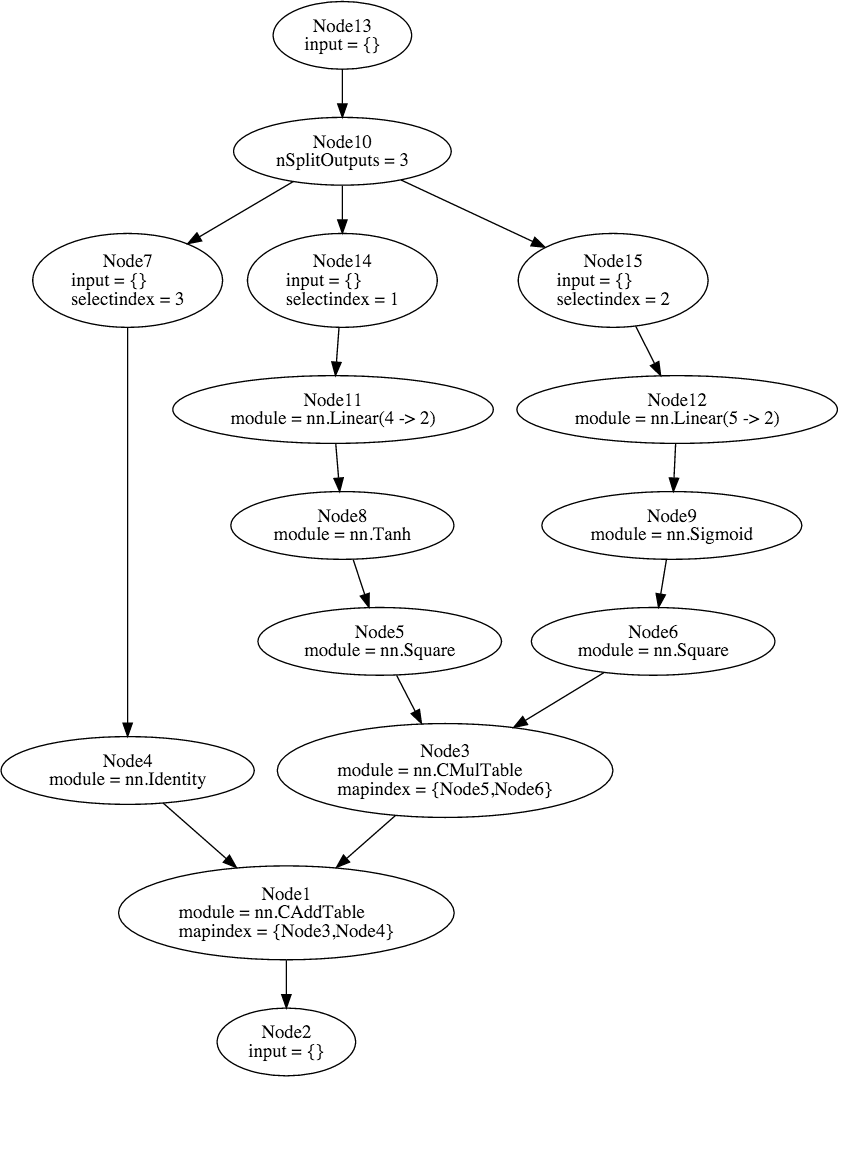
\includegraphics[width=0.40\textwidth]{warm}
  %\caption{ GRU cell graph\label{fig:gru_graph}}
%\end{figure}

\item See below the graph for the GRU cell.


\begin{figure}[ht!]
  \centering
  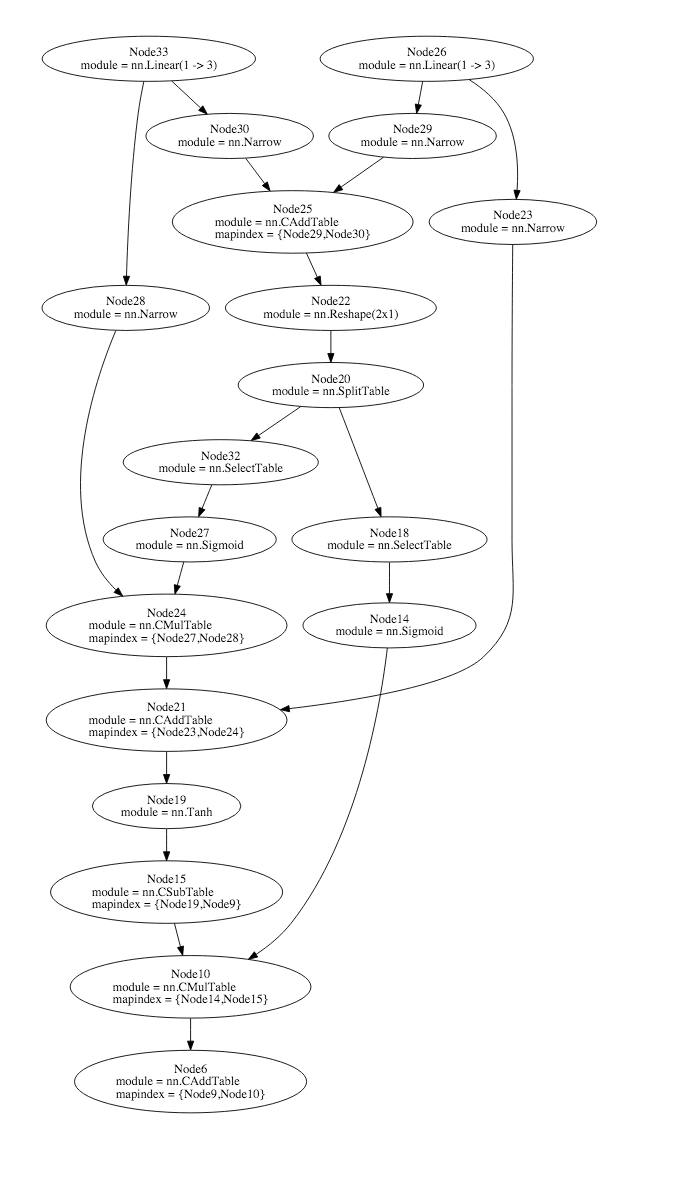
\includegraphics[width=0.60\textwidth]{GRU}
  \caption{ GRU cell graph\label{fig:gru_graph}}
\end{figure}
\end{itemize}

\section{Language modelling}
\subsection{Generating sequences}
The file query\_sentences.lua does the following thing:
\begin{enumerate}
  \item Load the network of the model
  \item Build the vocabulary map and the inverse vocabulary map.
  \item Get the number of words to predict and the number of words in the seed. 
  \item generate the index of each words doing a forward pass on the network, multinomial distribution over the probabilities generated by the logsoftmax layer. 
  \item Returns the new sentence.
\end{enumerate}
The code is in \cite{query}

\subsection{Suggested improvements to your model}
To improve the model I have tried a number of different thing:
\begin{itemize}
\item Change the number of layers from $2$ to $4$.
\item Change the size of the network from $100$ to $700$
\item Change the dropout parameter from $0$ to $0.5$
\item Change the vocabulary size from $10000$ to $12000$ 
\item Change the LSTM cell with the GRU cell
\item Change gradient clipping
\end{itemize}
 For the LSTM cell, the table below reports the best Perplexity and the parameters used.  The table is divided by a line. In the experiments below the line I use dropout  in the experiments above the line I didn't use it.
 When tuning the parameter I have noticed that an improvement in convergence speed and in the value of the perplexity occurred when augmenting the dropout parameter and simultaneously augmenting the size of the network. In particular the best model \cite{bestModel} has  rnn\_size$=600$ and  drop\_out$=0.4$, and it converges in about $8$ epochs to a value of Perplexity $~87.3$.
  

\begin{center}
\begin{tabular}{ |c|c|c|c|c|c|c|} 
\hline
seq length & layers & rnn size & dropout  & vocab size & best Perplexity\\
\hline
 20 & 2 & 200 & 0 &  10000 & 119.756\\ 
 30 & 2 & 200 & 0 &  10000 & 114.548\\ 
 15 & 2 & 200 & 0 &  10000 & 195.712\\ 
  30 & 4 & 200 & 0 & 10000 & 120.359\\
  40 & 3 & 200 & 0 & 15000 & 137.629\\
  \hline
 40 & 5 & 200 & 0.2 & 10000 & 135.020\\
 40 & 4 & 400 & 0.2 & 10000 & 107.970\\
 30 & 2 & 400 & 0.2 & 10000 & 93.449\\
 30 & 4 & 400 & 0.3 & 10000 & 102.013\\
  30 & 4 & 400 & 0.5 & 10000 & 113.420\\
  30 & 2 & 400 & 0.5 &  10000 & 96.340\\
  30 & 2 & 600 & 0.4 &  10000 & 87.368\\  
  30 & 2 & 500 & 0.3 &  10000 & 89.794\\  
\hline
\end{tabular}
\end{center}

The table below reports the value of the Perplexity and the parameters for models that use the GRU cell. As for the LSTM models I noticed an improvement using dropout along with an increasing size of the network. And I found that the best model for the GRU cell has the same parameter founded for the LSTM: rnn\_size$=600$ and  drop\_out$=0.4$. This model converges in about $11$ epochs to a value of Perplexity $~97.0$.


\begin{center}
\begin{tabular}{ |c|c|c|c|c|c|c|} 
\hline
seq length & layers & rnn size & dropout & vocab size & best Perplexity\\
\hline
 20 & 2 & 200 & 0 &  10000 & 182.217\\ 
 15 & 2 & 200 & 0 &  10000 & 195.712\\ 
 30 & 2 & 600 & 0.4 &  10000 & 97.056\\
 30 & 2 & 700 & 0.5 & 10000 & 101.021\\  
\hline
\end{tabular}
\end{center}
In the plot below I compered the best model for the LSTM and the best model for GRU plotting the Perplexity vs the Epoch. 





\begin{figure}[ht!]
  \centering
  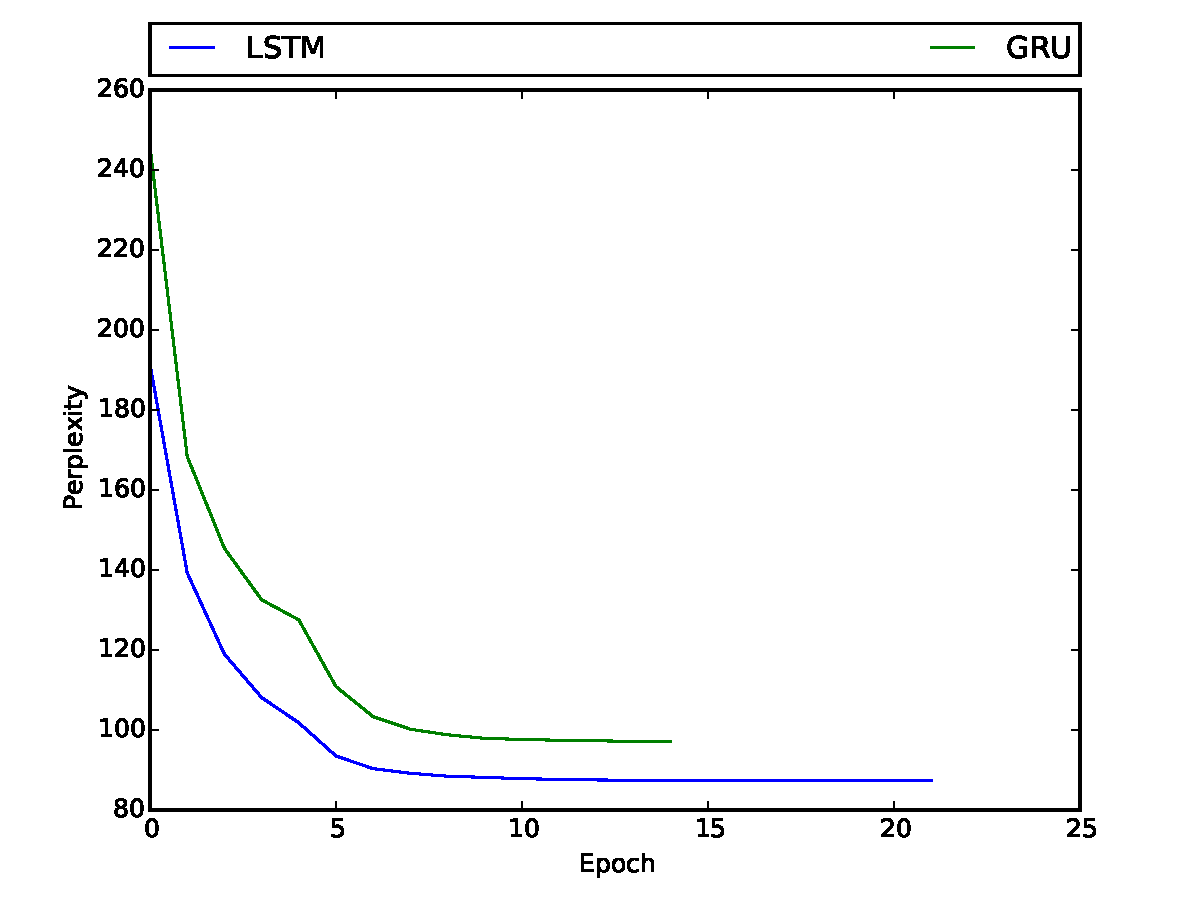
\includegraphics[width=1\textwidth]{LSTMvsGRU2.pdf}
  \caption{Comparison of the two best performing model for the LSTM cell (in blue) and for the GRU cell (in green)}
\end{figure}




\medskip

\small

%[1] Alexander, J.A.\ \& Mozer, M.C.\ (1995) Template-based algorithms
%for connectionist rule extraction. In G.\ Tesauro, D.S.\ Touretzky and
%T.K.\ Leen (eds.), {\it Advances in Neural Information Processing
%  Systems 7}, pp.\ 609--616. Cambridge, MA: MIT Press.



\begin{thebibliography}{9}
\bibitem{wormup} \url{https://github.com/mc3784/DL-A4/blob/master/submission/nngraph_warmup.lua}
\bibitem{query} \url{https://github.com/mc3784/DL-A4/blob/master/submission/query_sentences.lua}
\bibitem{bestModel} \url{http://cs.nyu.edu/~mc3784/model.net87.367553621956}
\bibitem{result}\url{https://github.com/mc3784/DL-A4/blob/master/submission/result.lua} 
\end{thebibliography} 




\end{document}


